
\documentclass[MASTER.tex]{subfiles} 
\begin{document} 
	

\begin{frame}
	\frametitle{Creating a Basic Plot}
	\vspace{-1cm}
	\Large
	\textbf{Creating a Basic Plot}
	\begin{itemize}
		\item To create a plot object we use the function \texttt{ggvis()}
		\item When we refer to variables in the data we use the
		`$\sim$` symbol before the name, i.e. \texttt{$\sim$ \texttt{Ozone}}
		\item We need to use a layer function, such as
		\texttt{layer\_points}, to plot the object.
	\end{itemize}
	
\end{frame}
%=================================================%
\begin{frame}[fragile]
	\begin{figure}
\centering
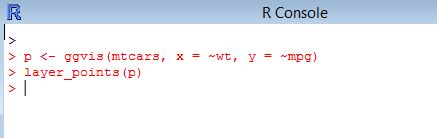
\includegraphics[width=0.99\linewidth]{images/basicscipt1}

\end{figure}
\Large
\begin{framed}
\begin{verbatim}
p <- ggvis(mtcars, x = ~wt, y = ~mpg)
layer_points(p)
\end{verbatim}
\end{framed}
\end{frame}
%=================================================%

\begin{frame}
(deprecated code?-  Watch out for this)
	\begin{figure}
\centering
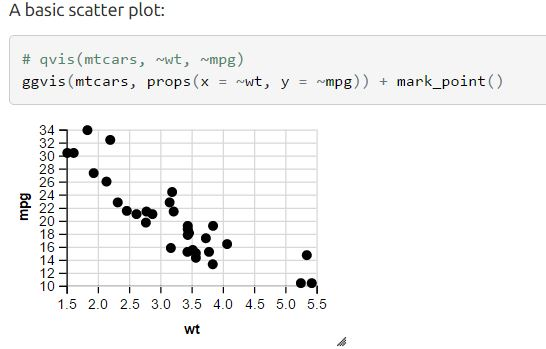
\includegraphics[width=1.05\linewidth]{plot01}
\end{figure}

\end{frame}
%==========================================================================%
\begin{frame}
	\frametitle{Data Visualization with ggvis}
	
	\Large
	\textbf{Web Graphics}
	\begin{itemize}
		\item You will notice that this plot opens in your \textbf{web browser} (unless you’re using RStudio). 
		\item That’s because all \textbf{ggvis} graphics are web graphics, and need to be shown in the web browser. \bigskip
		\item RStudio includes a built-in browser so it can show you the plots directly.
	
	\end{itemize}
	
\end{frame}
%================================================== %
%==========================================================================%
\begin{frame}[fragile]
	\frametitle{Data Visualization with ggvis}

	\Large
	\textbf{Code Legibility}\\
	\textit{Quoting Hadley Wickham}\\ 
\begin{itemize}
\item All ggvis functions take the visualisation as the first argument and return a modified visualisation.\item This seems a little bit awkward. \item Either you have to create temporary variables and modify them, or you have to use a lot of parentheses:
\end{itemize}

{
	\large
\begin{verbatim}
layer_points(ggvis(mtcars, x = ~wt, y = ~mpg))
\end{verbatim}
}
\end{frame}
%================================================== %

\end{document}